\documentclass{beamer}

% For more themes, color themes and font themes, see:
% http://deic.uab.es/~iblanes/beamer_gallery/index_by_theme.html
%
\mode<presentation>
{
  \usetheme{Madrid}       % or try default, Darmstadt, Warsaw, ...
  \usecolortheme{beaver} % or try albatross, beaver, crane, ...
  \usefonttheme{serif}    % or try default, structurebold, ...
  \setbeamertemplate{navigation symbols}{}
  \setbeamertemplate{caption}[numbered]
} 

\usepackage{tikz}
\usetikzlibrary{decorations.markings,angles}
\usepackage{tikz-3dplot} 

\usepackage{amsmath}


\begin{document}

\title[Two-fluid simulations]  
{Two-fluid simulations of solar partially ionized atmosphere }
\author[]{Beatrice Popescu Braileanu }
\institute[]{PhD advisors: \and \'Angel de Vicente \and %
                      Elena Khomenko}
\date{May 24, 2016}

\begin{frame}
\maketitle
\end{frame}

\begin{frame}[t]{Sun atmosphere layers}
\vspace*{-22pt}
\begin{columns}[b]
    \begin{column}{0.6\textwidth}
		Photosphere
        \begin{itemize}
					\item collisions dominated: LTE, MHD 
					\item	relatively easy observations 
					\item	diagnostics techniques well developed 
        \end{itemize}
    \end{column}
    \begin{column}{0.5\textwidth}
       % \rule{\textwidth}{0.75\textwidth}
			\begin{figure}[t]
			 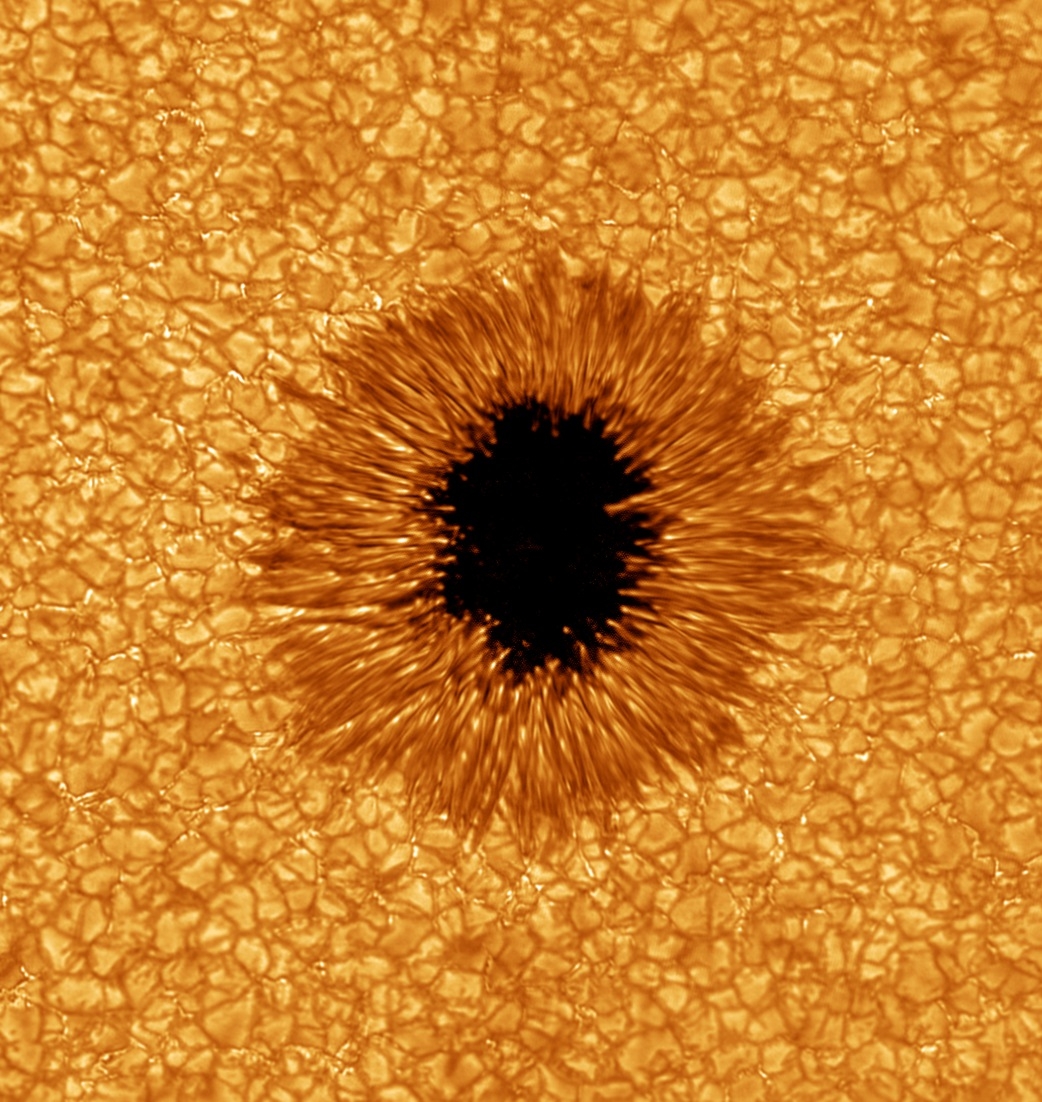
\includegraphics[scale=0.08]{phot.jpg}
			\end{figure}
    \end{column}
\end{columns}

\begin{columns}[b]
    \begin{column}{0.6\textwidth}
		Chromosphere
        \begin{itemize}
					\item not fully collisionally coupled: NLTE, No MHD (frequently not taken into account)
					\item very few spectral lines 
					\item complicated radiative diagostics 
        \end{itemize}
    \end{column}
    \begin{column}{0.5\textwidth}
       % \rule{\textwidth}{0.75\textwidth}
			\begin{figure}[t]
			 \centering
			 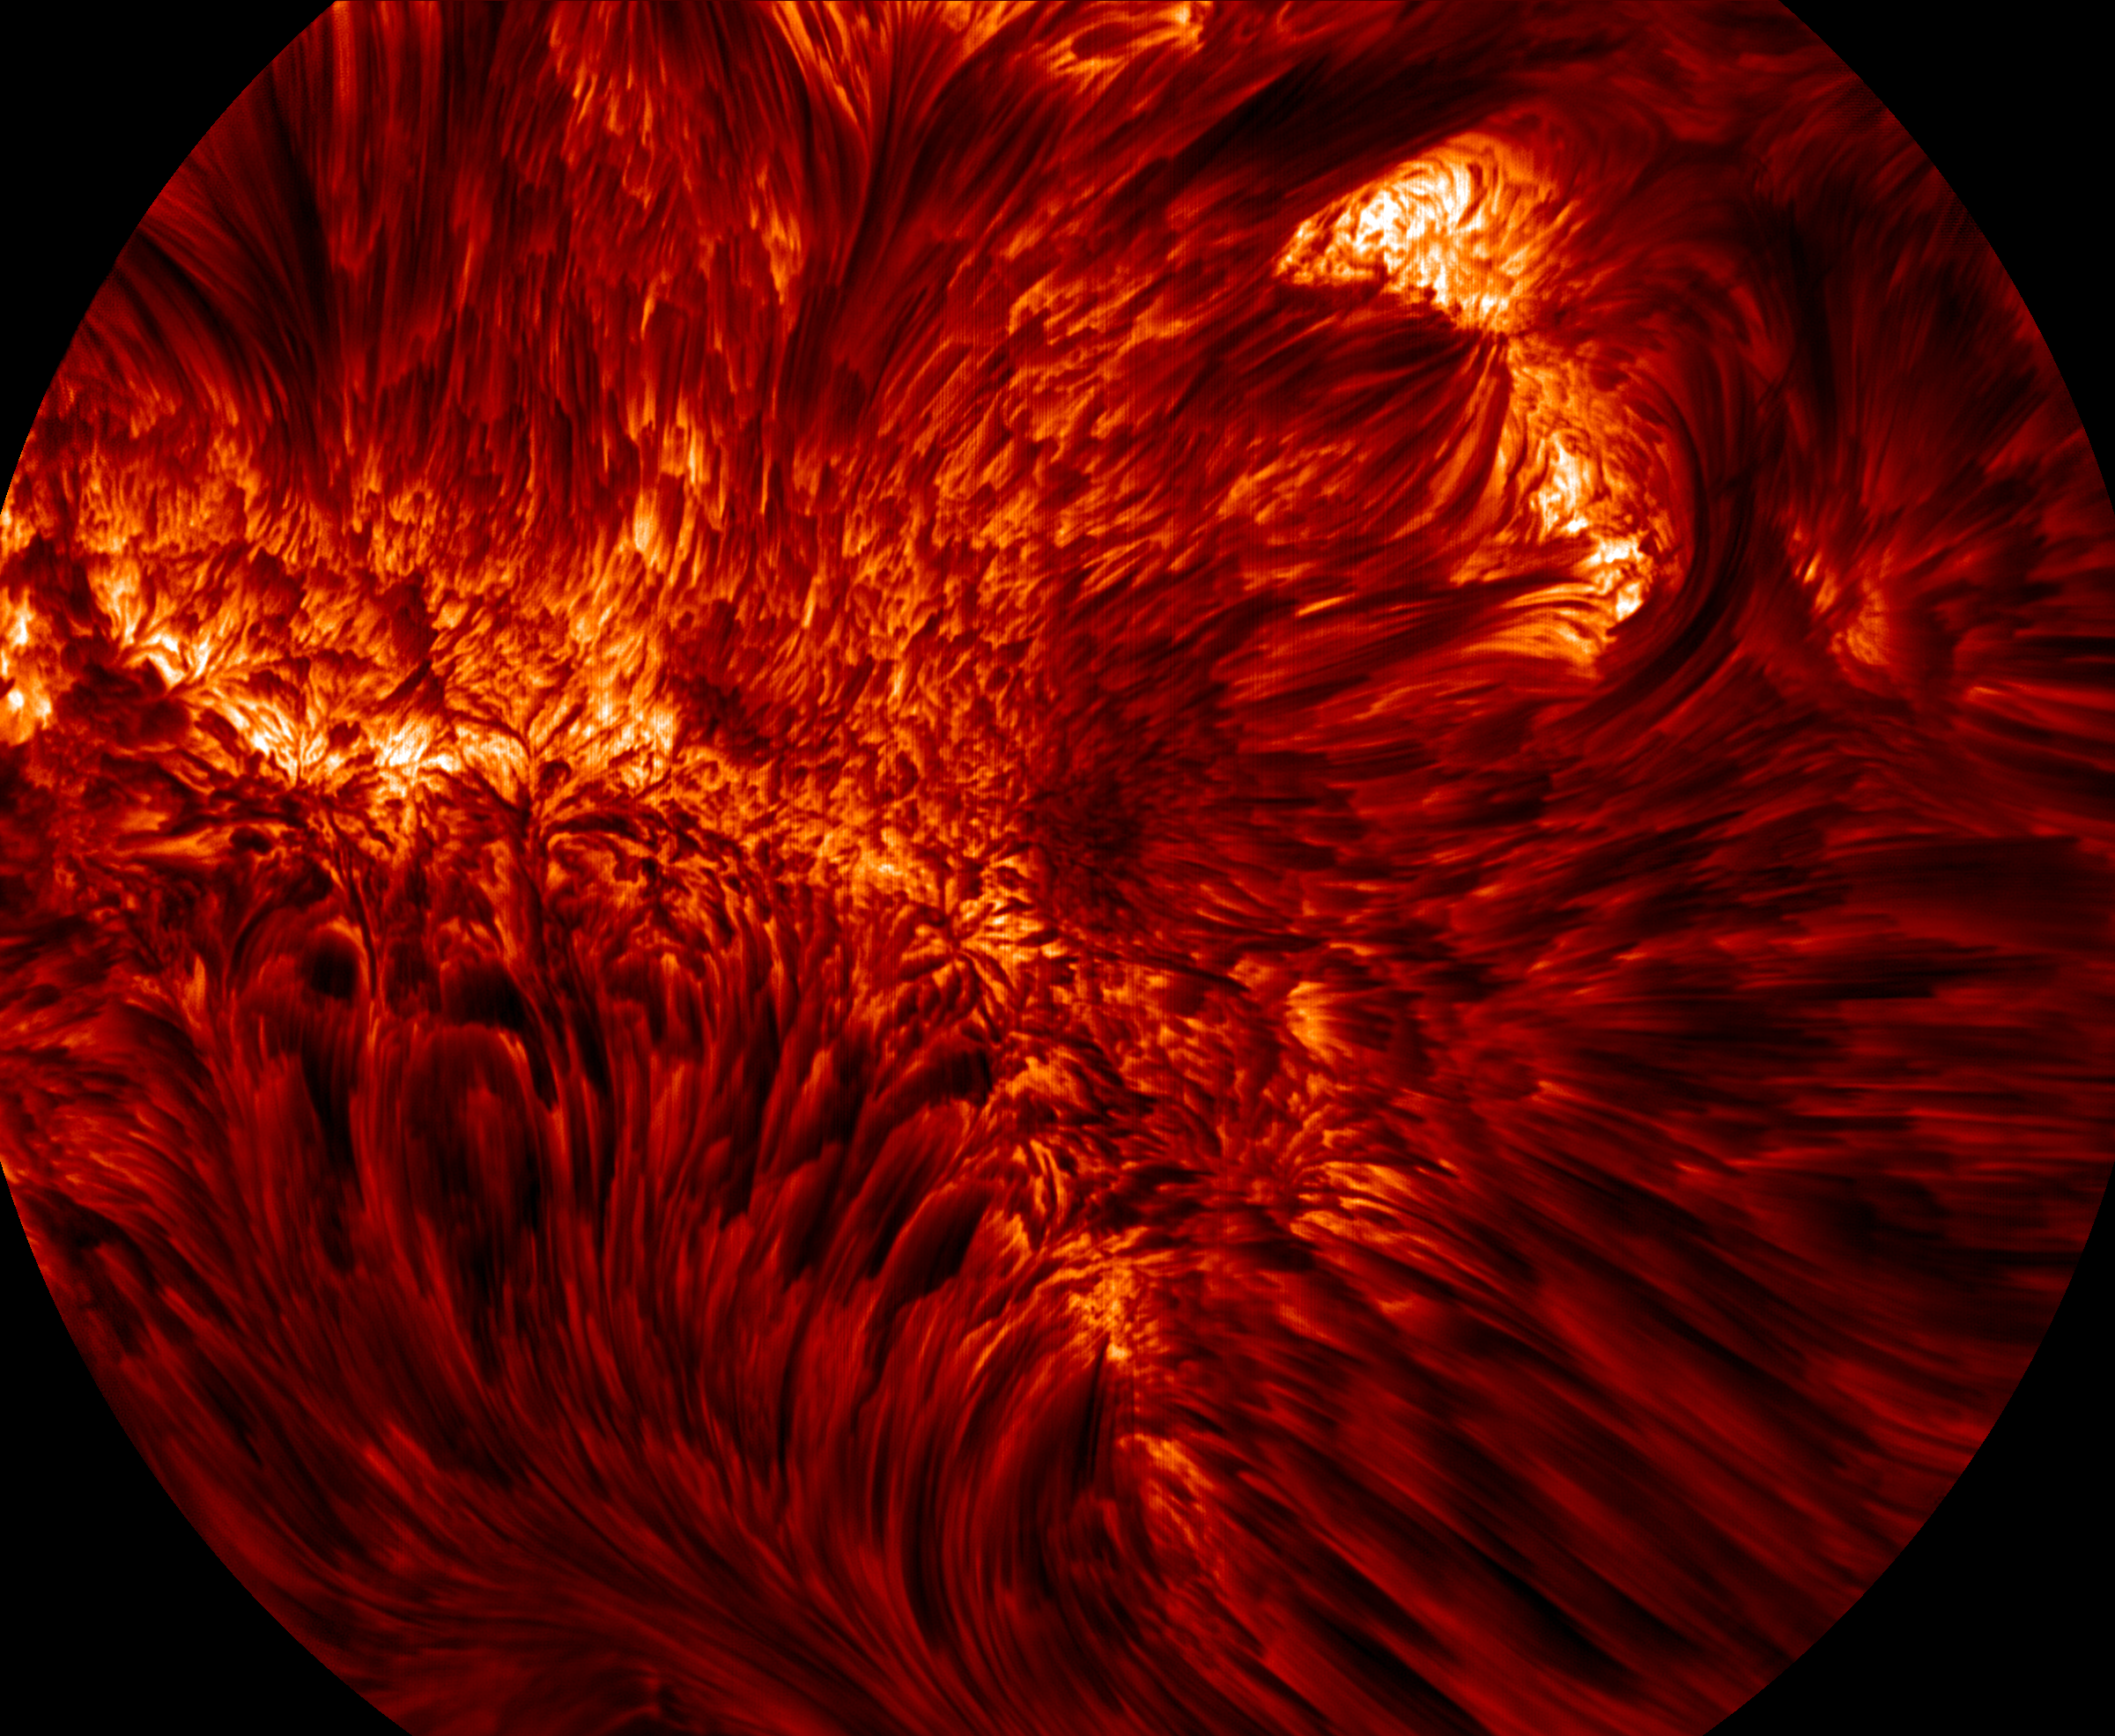
\includegraphics[scale=0.03]{chrom.png}
			\end{figure}
    \end{column}
\end{columns}

\begin{columns}[c]
    \begin{column}{0.6\textwidth}
		Corona
        \begin{itemize}
					\item magnetically dominated 
					\item very low density
					\item all ionized, MHD can be applied
        \end{itemize}
    \end{column}
    \begin{column}{0.5\textwidth}
			\begin{figure}[t]
			 \centering
			 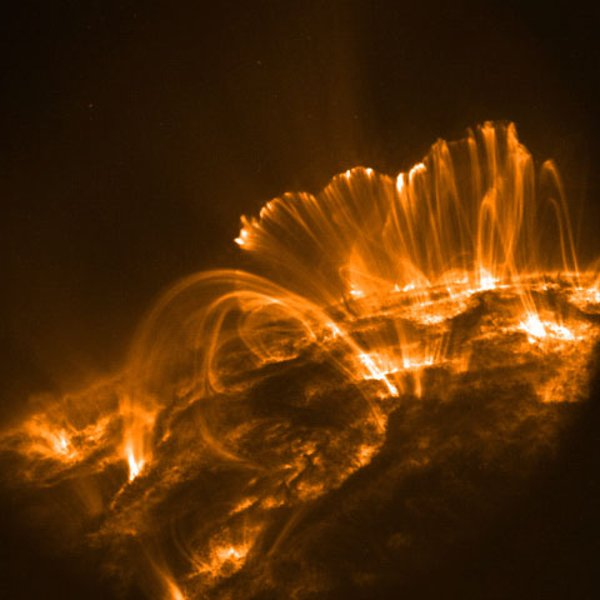
\includegraphics[scale=0.11]{corona.jpg}
			\end{figure}
    \end{column}
\end{columns}

\end{frame}

\begin{frame}{Plasma models}
\begin{itemize}
\item system of first order non linear partial differential equations which must be integrated in time
\item Approximations:
\begin{itemize}
\item MHD-1fluid: all the particles are considered as a whole. Assumption: strongly collisional plasma. A system of 8 unknown variables
($p,\rho,v_x,v_y,v_z,B_x,B_y,B_z$)
\item 2-fluid: Neutral particles do not feel electromagnetic forces and may move  differently from charged particles so collision rates between 
charged particles and neutral particles may not be the same like inside one specie. 
We consider the fluid variables ($p,\rho,v_x,v_y,v_z$) different for charged and neutral particles. A system of 13 unknown variables.
\item furthermore we could split the charges into ions and electrons as sometimes forces act differently on them or even consider each specie of ions
in order to gain more resolution over the process
\end{itemize}
\end{itemize}
\end{frame}

\begin{frame}{My work}
\begin{itemize}
\item including 2 fluid equations into  Mancha code
\begin{itemize}
\item fortran 90
\item parallelization with MPI
\item output in hdf5
\end{itemize}
\item making 2-fluid simulation
\begin{itemize}
\item generation of initial conditions (python)
\item executing the code
\item visualization  and analysis (visit or python)
\end{itemize}
\end{itemize}
\end{frame}

\begin{frame}{Test result in visit}
\begin{figure}[H]
 \centering
 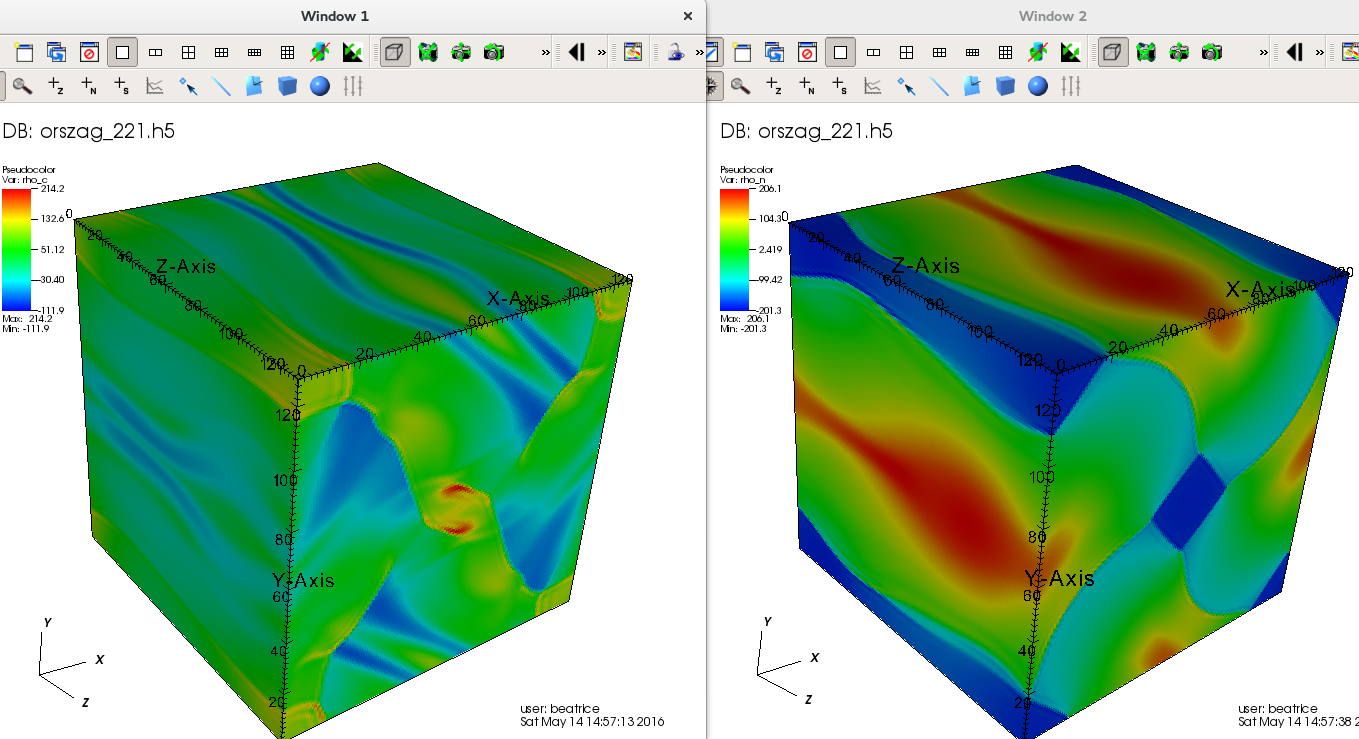
\includegraphics[scale=0.24]{visit2.png}
  \caption{density of charges and neutrals in Orszag test after 0.3836 s (221 iterations) where they evolve independently (collision terms between neutrals and charges are set to 0)}
\end{figure}
\end{frame}
\end{document}
